% !TEX root = Ragni2016.tex

% Disable review before sending
\documentclass[preprint, 12pt, a4paper,review]{elsarticle}

\usepackage[english]{babel}

\usepackage{amsmath}
\usepackage{amssymb}
\usepackage{pgf}
\usepackage[hidelinks]{hyperref}

\usepackage{lineno}
\usepackage{sty/tikz-uml}
\usetikzlibrary{arrows,automata}

% Code listing
\usepackage{xcolor,listings,fontspec,parcolumns}
\newfontfamily{\lstttfamily}[Scale=0.6]{Fira Mono}
\lstdefinestyle{customruby}{
  belowcaptionskip=0.3\baselineskip,
  breaklines=true,
  lineskip=-0.7ex,
  frame=tb,
  xleftmargin=\parindent,
  language=Ruby,
  showstringspaces=false,
  basicstyle=\lstttfamily\color{black},
  keywordstyle=\color{red!40!black},
  commentstyle=\color{gray},
  identifierstyle=\color{black},
  stringstyle=\color{green!40!black},
}
\lstloadlanguages{Ruby,Python,C}
\lstset{style=customruby}

% !TEX root = ../Ragni2016.tex

\newcommand{\reviewB}[1]{{\color{blue} #1}\xspace}
\newcommand{\review}[1]{{#1}\xspace}

\newcommand{\Ruby}{\emph{Ruby}\xspace}
\newcommand{\Mruby}{\emph{mRuby}\xspace}
\newcommand{\Jruby}{\emph{JRuby}\xspace}
\newcommand{\ragnicas}{\emph{Mr.CAS}\xspace}

%% Library command
\newcommand{\Array}{\texttt{Ar\-ray}}
\newcommand{\Float}{\texttt{Flo\-at}}
\newcommand{\Fixnum}{\texttt{Fix\-num}}

\newcommand{\Namespace}{\texttt{::}}

\newcommand{\CAS}{\texttt{CAS}}
\newcommand{\CASOp}{\CAS\Namespace\texttt{Op\-}}
\newcommand{\CASBinaryOp}{\CAS\Namespace\texttt{Bi\-na\-ry\-Op}}
\newcommand{\CASNaryOp}{\CAS\Namespace\texttt{Nary\-Op}}

\newcommand{\CASExpression}{\CAS\Namespace\texttt{Con\-di\-tion}}

\newcommand{\CASSin}{\CAS\Namespace\texttt{Sin}}
\newcommand{\CASSum}{\CAS\Namespace\texttt{Sum}}
\newcommand{\CASDiff}{\CAS\Namespace\texttt{Diff}}

\newcommand{\CASVariable}{\CAS\Namespace\texttt{Va\-ria\-ble}}
\newcommand{\CASConstant}{\CAS\Namespace\texttt{Con\-stant}}
\newcommand{\CASFunction}{\CAS\Namespace\texttt{Func\-tion}}
\newcommand{\CASPiecewise}{\CAS\Namespace\texttt{Piece\-wise}}

\newcommand{\CASOpsimplify}{\CASOp\texttt{\#sim\-pli\-fy}}
\newcommand{\CASOpsubs}{\CASOp\texttt{\#subs}}
\newcommand{\CASOpdiff}{\CASOp\texttt{\#diff}}
\newcommand{\CASOpcall}{\CASOp\texttt{\#call}}


\journal{SoftwareX}

\begin{document}

%  ___            _              _   _
% | __| _ ___ _ _| |_ _ __  __ _| |_| |_ ___ _ _
% | _| '_/ _ \ ' \  _| '  \/ _` |  _|  _/ -_) '_|
% |_||_| \___/_||_\__|_|_|_\__,_|\__|\__\___|_|
\begin{frontmatter}

\title{\ragnicas~- A Minimalistic (pure) \Ruby~CAS for Fast Prototyping and Code Generation}

\author[ragni]{Matteo Ragni}
\address[ragni]{Department of Industrial Engineering, University of Trento, 9, Sommarive, Povo di Trento, Italy}
\ead{matteo.ragni@unitn.it}

\begin{abstract}
There are complete \textbf{Computer Algebra System} (CAS) systems on the market with complete solutions for manipulation of analytical models. But exporting a model to a given target language is often a rigid procedure that requires some manual post-processing, even with a good software.
This work presents a \Ruby~library that exposes core CAS capabilities---i.e.\ simplification, substitution, evaluation, etc. The library aims at rapid prototyping of numerical interfaces, and code generation for different target languages, separating mathematical expression from code generation rules supporting best practices for numerical conditioning.
The library is implemented in pure \Ruby~language and is compatible with most \Ruby~interpreters.
\end{abstract}

\begin{keyword}
CAS \sep{} code-generation \sep{} Ruby
%% PACS codes here, in the form: \PACS code \sep code
%% MSC codes here, in the form: \MSC code \sep code
%% or \MSC[2008] code \sep code (2000 is the default)
\end{keyword}

\end{frontmatter}

\linenumbers{}

%% Body
% !TEX root = Ragni2016.tex

%  __  __     _   _          _   _
% |  \/  |___| |_(_)_ ____ _| |_(_)___ _ _
% | |\/| / _ \  _| \ V / _` |  _| / _ \ ' \
% |_|  |_\___/\__|_|\_/\__,_|\__|_\___/_||_|
\section{Motivation and significance}
\label{sec:motivation}

% Introduce the scientific background and the motivation for developing the software.
% Explain why the software is important, and describe the exact (scientific) problem(s) it solves.
% Indicate in what way the software has contributed (or how it will contribute in the future) to the
% process of scientific discovery; if available, this is to be supported by citing a research paper
% using the software.
% Provide a description of the experimental setting (how does the user use the software?).
% Introduce related work in literature (cite or list algorithms used, other software etc.).
\Ruby~\cite{flanagan2008ruby}~is a purely object-oriented scripting language designed in the mid-1990s by Yukihiro Matsumoto (also known as \emph{Matz}), internationally standardized since 2012 as ISO/IEC 30170.

With the advent of the \emph{Internet of Things}, a written from scratch version of the \Ruby~interpreter called \Mruby~(\emph{eMbedded Ruby})~\cite{tanaka2015mruby} has been published on \emph{GitHub} by Matsumoto, in 2014. The new interpreter is a lightweight implementation, aimed at both low power devices and PC, and complies with the standard\cite{iso30170}. \Mruby~has a completely new API, and it is designed to be embedded in complex projects as a front-end interface --- e.g.\ a numerical optimization suite may use \Mruby~to get problem input definitions.

The \Ruby~code-base exposes a large set of utilities in core and standard library, that can be furthermore expanded through modules, contained in \emph{gems}. Even if a high number of gems are deployed and available, there is no module that implements an \textbf{automatic symbolic differentiation} (ASD)~\cite{tolsma1998computational} engine that handles basic computer algebra routines, compatible with all different \Ruby~interpreters flavours.

\Ruby~has matured its fame as a web oriented language with \emph{Rails}, and can efficiently generate code in other languages. An ASD-capable gem is the foundamental step to rapidly develop specific code generators for well known software --- e.g.\ IPOPT~\cite{wachter2009ipopt}\@.

The module described in this work, is a gem implemented in pure \Ruby~code --- compatible with all standardized interpreters --- that is able to perform symbolic differentiation (SD) and some computer algebra operations~\cite{von2013modern}. The library aims at:
\begin{itemize}
  \item be an instrument for rapid development of prototype interface for numerical algorithms and exporting code generated in different target languages;
  \item generate rapidly descriptions of mathematical models, with \emph{easy to implement} conditioning rules for numerical issues, changing on request how the code is exported, and how expressions are formulated in the target language;
  \item \emph{separate mathematical expressions from numerical conditioning and workarounds};
  \item create a complete open-source CAS system for the standard \Ruby~language, as a long-term ambitious impact.
\end{itemize}

This is not the first gem that tries to implement a CAS.\@ The available computer algebra library for \Ruby~are:
\begin{description}
  \item [\emph{Rucas}~\cite{rucas}, \emph{Symbolic}~\cite{symbolic}] gems at early stage and with discontinued development status; they offer basic simplification routines. There is no differentiation method, but it is one of the milestones.
  \item [\emph{Symengine}~\cite{symengine}] is a wrapper for the C++ library \emph{symengine}. The back-end library is very complete, but it is compatible only with the RVM \Ruby~interpreter and has several dependencies. At the moment, the \emph{SciRuby}~\cite{sciruby}~project reports the gem as broken, and removed it from its codebase. From a direct test, when performing SD of an arbitrary function, the engine always returns \texttt{nil}.
\end{description}

%  ___                 _      _   _
% |   \ ___ ___ __ _ _(_)_ __| |_(_)___ _ _
% | |) / -_|_-</ _| '_| | '_ \  _| / _ \ ' \
% |___/\___/__/\__|_| |_| .__/\__|_\___/_||_|
%                       |_|
\section{Software description}
\label{sec:description}

% Describe the software in as much as is necessary to establish a vocabulary needed to explain
% its impact.

%    _          _    _ _          _
%   /_\  _ _ __| |_ (_) |_ ___ __| |_ _  _ _ _ ___
%  / _ \| '_/ _| ' \| |  _/ -_) _|  _| || | '_/ -_)
% /_/ \_\_| \__|_||_|_|\__\___\__|\__|\_,_|_| \___|
\subsection{Software Architecture}
\label{sec:architecture}

% Give a short overview of the overall software architecture; provide a pictorial component overview
% or similar (if possible). If necessary provide implementation details.

\ragnicas~is an object oriented AD gem that supports some simple computer algebra routines such as \emph{simplifications} and \emph{substitutions}. When gem is required, automatically overloads some methods of the \Fixnum~and \Float~classes, to make them compatible with the foundamental symbolic objects.

Each symbolic function is an object modeled by a class, that inherits from a common virtual ancestor: \CASOp (operation). An operation encapsulates sub-operations recursively, building a linked graph, that is the mathematical equivalent of function composition:
\begin{equation}
\left( f \, \circ \, g \right)
\end{equation}

\begin{figure}[ht!]
\label{fig:graph}
\centering
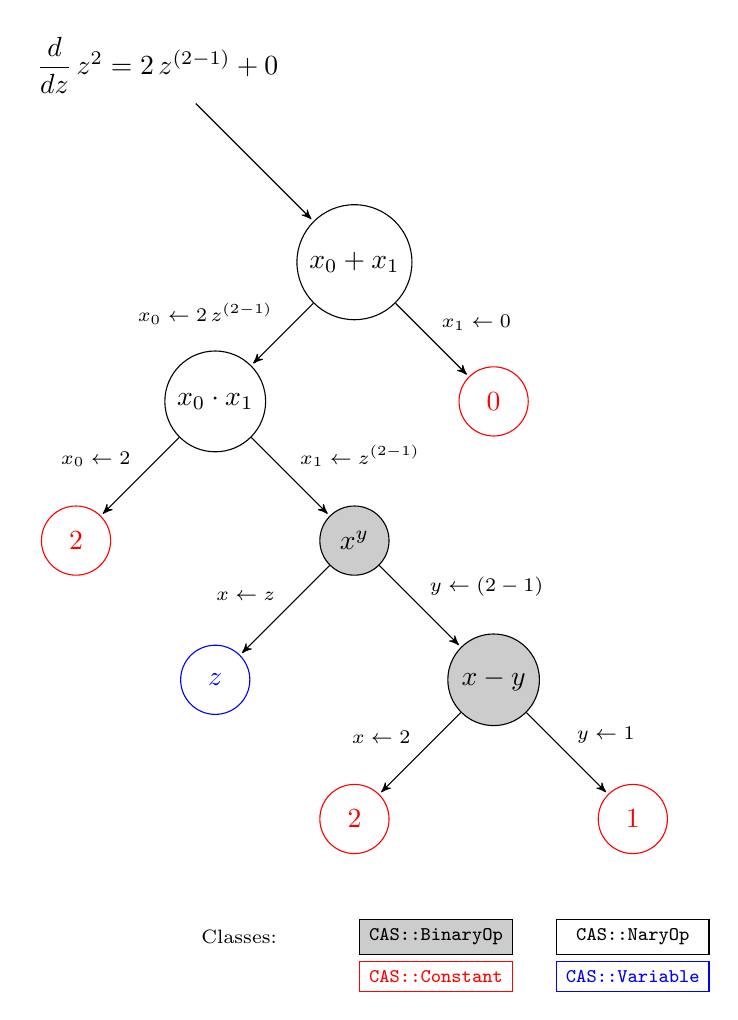
\begin{tikzpicture}[->,>=stealth',shorten >=1pt,auto,node distance=2.5cm]
  \tikzstyle{naryop}=[draw=black]
  \tikzstyle{constant}=[draw=red,text=red]
  \tikzstyle{variables}=[draw=blue,text=blue]
  \tikzstyle{binaryop}=[draw=black,fill=black!20]

  % Nodes
  \node[state]           (Sum)                          {$x_0 + x_1$};

  \node[state]           (Prod)  [below left of=Sum]    {$x_0 \cdot x_1$};
  \node[state,constant]  (Zero)  [below right of=Sum]   {$0$};

  \node[state,constant]  (Two)   [below left of=Prod]   {$2$};
  \node[state,binaryop]  (Pow)   [below right of=Prod]  {$x^y$};

  \node[state,variables] (X)     [below left of=Pow]    {$z$};
  \node[state,binaryop]  (Minus) [below right of=Pow]   {$x - y$};
  
  \node[state,constant]  (Two2)  [below left of=Minus]  {$2$};
  \node[state,constant]  (One)   [below right of=Minus] {$1$};
  
  % Legend
  \node[naryop]    (legend-Nary)   [below of=One,yshift=1cm] {\makebox[1.7cm]{\scriptsize\texttt{CAS::NaryOp}}};
  \node[binaryop]  (legend-Binary) [left of=legend-Nary]    {\makebox[1.7cm]{\scriptsize\texttt{CAS::BinaryOp}}};
  \node[variables] (legend-vars)   [below of=legend-Nary,yshift=2cm]     {\makebox[1.7cm]{\scriptsize\texttt{CAS::Variable}}};
  \node[constant]  (legend-const)  [left of=legend-vars]     {\makebox[1.7cm]{\scriptsize\texttt{CAS::Constant}}};
  \node (legendText) [left of=legend-Binary] {\scriptsize Classes:};

  % Origin
  \node (equation) [above of=Sum,xshift=-2.5cm] {$\dfrac{d}{dz}\,z^2 = 2\,z^{(2 - 1)}+0$};

  \path (Sum)      edge node [anchor=south east] {\scriptsize $x_0 \leftarrow 2\,z^{(2 - 1)}$} (Prod) 
                   edge node {\scriptsize $x_1 \leftarrow 0$}                                  (Zero)
        (Prod)     edge node [anchor=south east] {\scriptsize $x_0 \leftarrow 2$}              (Two)  
                   edge node                     {\scriptsize $x_1 \leftarrow z^{(2-1)}$}      (Pow)
        (Pow)      edge node [anchor=south east] {\scriptsize $x \leftarrow z$}                (X) 
                   edge node                     {\scriptsize $y \leftarrow (2 - 1)$}          (Minus)
        (Minus)    edge node [anchor=south east] {\scriptsize $x \leftarrow 2$ }               (Two2) 
                   edge node                     {\scriptsize $y \leftarrow 1$ }               (One)
        (equation) edge                                                                        (Sum);
\end{tikzpicture}
\caption{Example graph from the first function reported in listing~\ref{code:example-diff}}
\end{figure}

When a new operation is created, it is appended to the graph. The number of branches are determined by the parent container class of the current symbolic function. There are three possible containers. Single argument functions --- e.g. $\sin(\cdot)$ --- have as closest parent the \CASOp~class, that links to one sub-graph. Functions with two arguments --- e.g.\ difference or exponential function --- inherit from \CASBinaryOp, that links to two subgraphs. Functions with arbitrary number of arguments --- e.g.\ sum and product --- have as parent the \CASNaryOp\footnote{Please note that this container is still at experimental stage}, that links to an arbitrary number of subgraph. Figure~\ref{fig:graph} contains an example of graph. The different kind of containers allows to introduce some properties like \emph{associativity} and \emph{commutativity}. Each container exposes the subgraphs as instance properties. Containers structure is shown in Figure~\ref{fig:uml-container}.

Terminal leaf of the graph are the two classes \CASConstant~and \CASVariable. The first is a node for a simple numerical value, while the latter represents an independent variable, that can be used to perform derivatives and evaluations. As for now, those nodes are only scalar numbers, with plans to define also the vectorial and matricial extensions in the next major release.

Automatic differentiation (\CASOpdiff) crosses the graph until it reaches the ending node. The terminal node is the starting point for derivatives accumulation, the mathematical equivalent of the chain rule:
\begin{equation}
\left( f  \, \circ \, g \right)' \: = \:
\left( f' \, \circ \, g \right) \: g'
\end{equation}
The recursiveness is used also for simplifications (\CASOpsimplify), substitutions (\CASOpsubs) and evaluations (\CASOpcall).

\begin{figure}[ht!]
\label{fig:uml-container}
\centering
\begin{tikzpicture}
\umlclass[type=abstract]{CAS::Op}{
x : CAS::Op
}{
\umlvirt{ diff(CAS::Op) : CAS::Op } \\
\umlvirt{ subs(Hash) : CAS::Op    } \\
\umlvirt{ call(Hash) : Numeric } \\
\umlvirt{ simplify : CAS::Op      }
}

\umlclass[type=abstract,x=3,y=-5.5]{CAS::BinaryOp}{
x : CAS::Op \\
y : CAS::Op
}{}

\umlclass[type=abstract,x=3,y=-10.5]{CAS::NaryOp}{
x : Array
}{}

\umlemptyclass[x=8]{CAS::Sin}
\umlemptyclass[x=8,y=-2]{CAS::Log}
\umlsimpleclass[x=8,y=-3.5,draw=white]{...}

\umlemptyclass[x=8,y=-5.5]{CAS::Diff}
\umlemptyclass[x=8,y=-7.5]{CAS::Pow}
\umlsimpleclass[x=8,y=-9,draw=white]{...}

\umlemptyclass[x=8,y=-10.5]{CAS::Sum}
\umlemptyclass[x=8,y=-12.5]{CAS::Mul}
\umlsimpleclass[x=8,y=-14,draw=white]{...}


% Inheritance
\umlinherit[geometry=|-,anchor2=west]{CAS::Op}{CAS::BinaryOp}
\umlinherit[geometry=|-,anchor2=west]{CAS::Op}{CAS::NaryOp}

\umlinherit[geometry=--,anchor1=east,anchor2=west]{CAS::Op}{CAS::Sin}
\umlinherit[geometry=-|-,anchor1=east,anchor2=west]{CAS::Op}{CAS::Log}

\umlinherit[geometry=--,anchor1=east,anchor2=west]{CAS::BinaryOp}{CAS::Diff}
\umlinherit[geometry=-|-,anchor1=east,anchor2=west]{CAS::BinaryOp}{CAS::Pow}

\umlinherit[geometry=--,anchor1=east,anchor2=west]{CAS::NaryOp}{CAS::Sum}
\umlinherit[geometry=-|-,anchor1=east,anchor2=west]{CAS::NaryOp}{CAS::Mul}

\end{tikzpicture}

\caption{Simplified version of classes interface and inheritance}
\end{figure}

%  ___             _   _               _ _ _   _
% | __|  _ _ _  __| |_(_)___ _ _  __ _| (_) |_(_)___ ___
% | _| || | ' \/ _|  _| / _ \ ' \/ _` | | |  _| / -_|_-<
% |_| \_,_|_||_\__|\__|_\___/_||_\__,_|_|_|\__|_\___/__/
\subsection{Software Functionalities}
\label{sec:functionalities}

\subsubsection{Basic Functionalities}
% Present the major functionalities of the software.
The main functionality of the library is the \textbf{AD}, that can be performed with respect to an independent variable (\CASVariable), even for implicit functions. The differentiation is done by a method of the \CASOp, having a \CASVariable~as argument:
\begin{lstlisting}[caption={Differentiation example},label={code:example-diff}]
x = CAS.vars 'x'           # creates a variable
f = x ** 2 + 1             # define a symbolic expression
f.diff(x)                  # derivative w.r.t. x
# => 2 * x ^ (2 - 1) + 0
g = CAS.declare :g, f      # creates implicit function
g.diff(x)                  # derivative w.r.t. x
# => (x ^ (2 - 1) * 2) * Dg[0](x ^ 2)
\end{lstlisting}

Resulting graph still contains a zero, since \textbf{simplifications} are not executed automatically. Each node of the graph contains some rules for simplify itself. Simplification are called recursively inside the graph, exactly like AD, bringing the strong limitation of not handling simplifications that come from \emph{heuristic expansion} of sub-graphs --- e.g.\ simplification through the use of trigonometric identities. Those simplification can be achieved manually using \textbf{substitutions}.
\begin{lstlisting}[caption={Simplification example},label={code:example-simp}]
x, y = CAS::vars 'x', 'y'        # creates two variables
f = CAS.log( CAS.sin( y ) )      # symbolic expression
f.subs  y: CAS.asin(CAS.exp(x))  # perform substitution
f.simplify                       # simplify expression
# => x
\end{lstlisting}

The graph can be \textbf{evaluated} substituting defining some values for the independent variable in a feed dictionary. The graph is recursively reduced to a single numeric value:
\begin{lstlisting}[caption={Graph evaluation example},label={code:example-call}]
\label{code:example-call}
x = CAS::vars 'x'          # creates a variable
f = x ** 2 + 1             # define a symbolic expression
f.call x => 2                # evaluate for x = 2
# => 5
\end{lstlisting}

Symbolic functions can be used to create expressions --- e.g. $f(\cdot) \geq g(\cdot)$ --- or piecewise functions --- e.g. $\max(f(\cdot), g(\cdot))$:
\begin{lstlisting}[caption={Expressions and Piecewise functions},label={code:example-expr}]
x = CAS::vars 'x'
f = x ** 2
g = 2 * x + 1
f.greater_equal g
# => ((x)^(3) >= ((2 * x) + 1))
CAS::max f, g
# => (((x)^(3) >= ((2 * x) + 1)) ? (x)^(3) : ((2 * x) + 1))
\end{lstlisting}
Expression are stored in a special container class, called \CASExpression.

\subsubsection{Metaprogramming and Code-Generation}

The library is developed explicitly for \textbf{generation of code}, and in some case also \textbf{meta\-programming}. Expressions, once manipulated, can be easily exported as source code (in a defined language ---i.e. the following example in standard \Ruby~code) the function is used as a prototype for a callable \emph{closure} (\texttt{Proc} object):
\begin{lstlisting}[caption={Graph evaluation example},label={code:example-proc}]
x = CAS::vars 'x'             # creates a variable
f = CAS::log(CAS::sin(x))     # define a symbolic function

proc = f.as_proc              # exports callable lambda
proc.call 'x' => Math::PI/2
# => 0.0
\end{lstlisting}
Must be noted that making a closure of the graph is like making a snapshot, and any further modifications to the graph will not update the callable object. This drawback is balanced by faster execution time of the \texttt{Proc}: when a graph needs only to be evaluated in a iterative algorithm, and not to be manipulated, transforming it in a \emph{closure} reduces the execution time per loop.

Code generation should be flexible enough to export a graph in a user's target language. Generation functions are usually included in specific plugins. Users can expand exporting capabilites by writing specific exportation rules,  overriding method when required, or describing their own plugin:
\begin{lstlisting}[caption={Example of Ruby exportation plugin},label={code:example-exporting}]
# Definition
module CAS
  {
    # . . .
    CAS::Variable => Proc.new { "#{name}" }
    CAS::Sin      => Proc.new { "Math.sin(#{x.to_ruby})" },
    # . . .
  }.each do |cls, prc|
    cls.send(:define_method, :to_ruby, &prc)
  end
end

# Usage
x = CAS.vars 'x'
(CAS.sin(x)).to_ruby
# => Math.sin(x)
\end{lstlisting}

Included plugins may implement some advanced features such as code optimization: this is an example with the \emph{C} plugin:

\begin{lstlisting}[caption={Calling optimized-C exporter},label={code:example-exporting-C-1}]
require 'ragni-cas/c-opt'

x, y = CAS.vars :x, :y
f = x ** y + CAS.log(CAS.sin(x ** y))

CLib.create "example" do
  implements_as "func", f
end
\end{lstlisting}
library created contains the following source (the header is omitted for brevity):
\begin{lstlisting}[caption={Calling optimized-C exporter},label={code:example-exporting-C-2},language=C]
  // Source file for library: example.c

  #include "example.h"

  double func(double x, double y) {
    double __t_0 = pow(x, y);
    double __t_1 = sin(__t_0);
    double __t_2 = log(__t_1);
    double __t_3 = (__t_0 + __t_2);

    return __t_3;
  }

  // end of example.c
\end{lstlisting}

%  ___      _                _
% / __|_ _ (_)_ __ _ __  ___| |_ ___
% \__ \ ' \| | '_ \ '_ \/ -_)  _(_-<
% |___/_||_|_| .__/ .__/\___|\__/__/
%            |_|  |_|
%\subsection{Sample code snippets analysis (optional)}
%\label{sec:snippets}

%  ___                     _
% | __|_ ____ _ _ __  _ __| |___ ___
% | _|\ \ / _` | '  \| '_ \ / -_|_-<
% |___/_\_\__,_|_|_|_| .__/_\___/__/
%                    |_|
\section{Illustrative Examples}
\label{sec:examples}

\subsection{Code Generation as C Library}
This example shows how to export a C library using the \texttt{CAS} module as design interface. \texttt{c-opt} plugin implements advanced features such as code optimization and generation of libraries.

In this example we create a library \texttt{example} that implements the model:

\begin{equation}
f(x, y) = x^y + g(x)\, \mathrm{log}(\sin(x^y))
\end{equation}

Expression $g(x)$ is implemented as \texttt{g\_impl} and its interface is described in the external header \texttt{g\_impl.h}. The code must be optimized: the intermediate operation $x^y$ should be evaluated once, even if required twice in our model. The C function that implements our model $f(x,y)$ should be called with the token \texttt{f\_impl}. The exporter uses as default type, for variables and function returned values, \texttt{double}.

\begin{lstlisting}[caption={Calling optimized-C exporter for library generation},label={code:example-exporting-C-1}]
require 'ragni-cas/c-opt'

# Models
x, y = CAS.vars :x, :y
g = CAS.declare :g, x

f = x ** y + g * CAS.log(CAS.sin(x ** y))

# Code Generation
g.c_name = 'g_impl'             # g token

CAS::CLib.create "example" do
  include_local "g_impl"        # g header
  implements_as "f_impl", f     # token for f
end
\end{lstlisting}
Library created by class \texttt{CLib} contains the following code:

\noindent%
  \begin{minipage}{.5\textwidth}
    \lstinputlisting[style=customruby,language=C,caption={C Header}]{./scripts/source.h}
  \end{minipage}\hfill
  \begin{minipage}{.5\textwidth}
    \lstinputlisting[style=customruby,language=C,caption={C Source},frame=tbl]{./scripts/source.c}
  \end{minipage}

\subsection{Using the module as interface}
As example, an implementation of an algorithm that extimates the \emph{order of convergence} for trapezoidal integration scheme \cite{weideman2002numerical} is provided, using the automatic differentiation as interface.

Given a function $f(x)$, the trapezoidal rule for primitive estimation in the interval $[a,\,b]$ is:
\begin{equation}
  I_{n}(a, b) = \dfrac{b - a}{n} \left( \dfrac{f(a) + f(b)}{2} +
    \sum\limits_{k = 1}^{n - 1}{f \left( a + k \dfrac{b - a}{n} \right)} \right)
\end{equation}
where $n$ mediates the integration's step size. When exact primitive $F(x)$ is known, approximation error is:
\begin{equation}
  E[n] = F(b) - F(a) - I_{n}(a, b)
\end{equation}
This error shows a direct relation:
\begin{equation}
  E[n] \propto C\,{n}^{-p}
\end{equation}
where $p$ is the convergence order. Using a different value for $n$, for example $2\,n$:
\begin{equation}
  \dfrac{E[n]}{E[2\,n]} \approx 2^{p} \quad \rightarrow \quad p \approx log_2 \left( \dfrac{E[n]}{E[2\,n]} \right)
\end{equation}
Following listings contain the implementation of the described procedure using the described gem and the well known \emph{Python} \cite{van2011python} library \emph{sympy} \cite{christopher_smith_2016_47274}.

\noindent%
  \begin{minipage}{.5\textwidth}
    \lstinputlisting[style=customruby,caption={Ruby version}]{./scripts/test.rb}
  \end{minipage}\hfill
  \begin{minipage}{.5\textwidth}
    \lstinputlisting[style=customruby,language=python,caption={Python version},frame=tbl]{./scripts/test.py}
  \end{minipage}

% !TEX root = Ragni2016.tex

%  ___                     _
% |_ _|_ __  _ __  __ _ __| |_
%  | || '  \| '_ \/ _` / _|  _|
% |___|_|_|_| .__/\__,_\__|\__|
%           |_|
\section{Impact}
\label{sec:impact}

% \textbf{This is the main section of the article and the reviewers weight the description here appropriately}
% Indicate in what way new research questions can be pursued as a result of the software (if any).
% Indicate in what way, and to what extent, the pursuit of existing research questions is improved (if so).
% Indicate in what way the software has changed the daily practice of its users (if so).
% Indicate how widespread the use of the software is within and outside the intended user group.
% Indicate in what way the software is used in commercial settings and/or how it led to the creation
% of spin-off companies (if so).
\ragnicas~is a midpoint between a CAS and an ASD library. It allows to manipulate expressions while mantaining the complete control on how the code is exported. Each rule is overloaded and applied runtime, without the need of compilation. Each user's model may include the mathematical description, code generation rules and high level logic that should be intrisic to such a rule --- e.g.~exporting gradients as \textbf{patterns} instead of matrices.

Our research group is including \texttt{Mr.CAS} in a solver for optimal control problem with indirect methods, as interface for problems' description~\cite{biral2016notes}.

As a long term ambitious impact, this library will become a complete CAS for \Ruby~language, filling the empty space reported by \emph{SciRuby} for symbolic math engines.

% !TEX root = Ragni2016.tex

%   ___             _         _
%  / __|___ _ _  __| |_  _ __(_)___ _ _  ___
% | (__/ _ \ ' \/ _| | || (_-< / _ \ ' \(_-<
%  \___\___/_||_\__|_|\_,_/__/_\___/_||_/__/
\section{Conclusions}
\label{sec:conclusions}

% Set out the conclusion of this original software publication.
This work presents a pure \Ruby~library that implements a minimalistics CAS with
automatic and symbolic differentiation that is aimed at code generation or metaprogramming.
The library is still at an early developing stage, but with promising feature, some of them
shown in section~\ref{sec:examples}. This is the only gem that implements
such a functionality for this language.

Language features allows to use library as an interface, simplifying model definition
for numerical algorithms. All core functionalities and basic math are defined, with the plan to expand
capabilities furthemore as milestones for next major releases. Reopening a class guarantees a
\emph{liquid} library 

Library is published in repository \emph{rubygems.org} and versioned on \emph{github.com}. It can be included easily in projects and in inline interpreter, or installed as a standalone gem.


\section*{Acknowledgements}
\label{sec:acknowledgements}
This research did not receive any specific grant from funding agencies in the public, commercial, or not-for-profit sectors.

%  ___ _ _    _ _                         _
% | _ |_) |__| (_)___  __ _ _ _ __ _ _ __| |_ _  _
% | _ \ | '_ \ | / _ \/ _` | '_/ _` | '_ \ ' \ || |
% |___/_|_.__/_|_\___/\__, |_| \__,_| .__/_||_\_, |
%                     |___/         |_|       |__/
\bibliographystyle{elsarticle-num}
\bibliography{bib}


% !TEX root = ../Ragni2016.tex

% __   __          _          _
% \ \ / /__ _ _ __(_)___ _ _ (_)_ _  __ _
%  \ V / -_) '_(_-< / _ \ ' \| | ' \/ _` |
%   \_/\___|_| /__/_\___/_||_|_|_||_\__, |
%                                   |___/
\section*{Current code version}
\label{sec:version-dev}

% Ancillary data table required for subversion of the codebase. Kindly replace examples in
% right column with the correct information about your current code, and leave the left column
% as it is.

\begin{table}[!h]
\begin{tabular}{|l|p{6.5cm}|p{6.5cm}|}
\hline
\textbf{Nr.} & \textbf{Code metadata description} & \textbf{Please fill in this column} \\
\hline
C1 & Current code version & 0.2.7 \\
\hline
C2 & Permanent link to code/repository used for this code version & \href{https://github.com/ElsevierSoftwareX/SOFTX-D-17-00013}{github.com/ ElsevierSoftwareX/SOFTX-D-17-00013} \\
\hline
C3 & Legal Code License   & MIT\\
\hline
C4 & Code versioning system used & \emph{git} (GitHub)\\
\hline
C5 & Software code languages, tools, and services used & \Ruby~language\\
\hline
C6 & Compilation requirements, operating environments & \Ruby~$\geq 2.x$\\
\hline
C7 & If available Link to developer documentation/manual & \href{http://www.rubydoc.info/gems/Mr.CAS}{rubydoc.info/gems/Mr.CAS} \\
\hline
C8 & Support email for questions & \href{mailto:info@ragni.me}{info@ragni.me} \\
\hline
\end{tabular}
\caption{Code metadata (mandatory)}
\label{tab:code-metadata}
\end{table}

% \section*{Current executable software version}
% \label{sec:version-gem}
%
% % Ancillary data table required for sub version of the executable software: (x.1, x.2 etc.)
% % kindly replace examples in right column with the correct information about your executables,
% % and leave the left column as it is.
%
% \begin{table}[!h]
% \begin{tabular}{|l|p{6.5cm}|p{6.5cm}|}
% \hline
% \textbf{Nr.} & \textbf{(Executable) software metadata description} & \textbf{Please fill in this column} \\
% \hline
% S1 & Current software version & 0.0.0 \\
% \hline
% S2 & Permanent link to executables of this version  & \href{https://rubygems.org/gems/ragni-cas}{rubygems.org/gems/ragni-cas} \\
% \hline
% S3 & Legal Software License & MIT \\
% \hline
% S4 & Computing platforms/Operating Systems & x86, amd64, arm-hf, mips/Windows, Linux, OS-X \\
% \hline
% S5 & Installation requirements \& dependencies & \Ruby $\geq 2.x$, \emph{pry} gem for console (optional)\\
% \hline
% S6 & If available, link to user manual - if formally published include a reference to the publication in the reference list & Wiki not yet ready: \href{https://github.com/MatteoRagni/cas-rb/wiki/Welcome}{Project's Wiki} \\
% \hline
% S7 & Support email for questions & \href{mailt:info@ragni.me}{info@ragni.me} \\
% \hline
% \end{tabular}
% \caption{Software metadata (optional)}
% \label{}
% \end{table}

\end{document}
\endinput

%%
%% End of file `Ragni2016.tex'.
